\documentclass[10pt,twocolumn]{article}

\usepackage[margin=0.72in]{geometry}
\usepackage{graphicx}
\usepackage{booktabs}
\usepackage{amsmath}
\usepackage{amssymb}
\usepackage{url}
\usepackage{hyperref}
\usepackage{caption}
\usepackage{subcaption}
\usepackage{xcolor}

\hypersetup{colorlinks=true, linkcolor=black, citecolor=black, urlcolor=blue}

\title{\vspace{-1.0em}Q-ORACLE: A Hardware-Backed Temporal Quantum Machine Learning Pipeline for PESTEL Scenario Forecasting}
\author{Yehor Tereshchenko \\ QuantumFinances / Q-ORACLE Prototype}
\date{June 2026}

\begin{document}
\maketitle

\begin{abstract}
We present Q-ORACLE, a prototype pipeline that extends weekly news-graph foresight into a compact temporal quantum machine learning (QML) experiment. The system starts from ORACLE-style time-dependent recursive summary graph snapshots, extracts weekly PESTEL vectors, forms event-conditioned future scenario targets, trains a small variational quantum circuit on week-to-week transitions, and submits the learned inference circuit to IQM Sirius hardware. The current experiment uses three weekly graph snapshots, a four-qubit temporal latent encoding, two layers of variational rotations and entanglement, and a two-bit scenario readout. A verified IQM temporal-QML job returned 128 hardware shots with counts \(\{00:53,01:26,10:32,11:17\}\), corresponding to a sampled distribution over stable, aligned-up, aligned-down and uncertain branches. We position the result as a reproducible hardware-backed systems demonstration rather than evidence of predictive market validity. The contribution is an end-to-end, inspectable method for connecting auditable news foresight, PESTEL world-state vectors and near-term quantum processors.
\end{abstract}

\section{Introduction}
News-driven foresight systems are useful only when they preserve traceability from raw evidence to the resulting strategic interpretation. ORACLE-style time-dependent recursive summary graphs (TRSGs) address this by converting news streams into weekly clustered graph snapshots, summarizing them recursively, and grounding interpretation in PESTEL dimensions. The reference ORACLE paper frames this as an auditable foresight layer rather than an opaque prediction engine~\cite{oracle2025}.

Q-ORACLE asks a narrower experimental question: can the weekly PESTEL trajectory produced by such a foresight system be converted into a small temporal QML task and executed on real quantum hardware? The goal is not to claim financial prediction or quantum advantage. Instead, the goal is to make the whole chain concrete enough for inspection: graph snapshots become vectors, vectors become training pairs, training pairs define a variational circuit, and the trained inference circuit is sampled on a quantum processing unit (QPU).

The resulting prototype runs as a standalone backend/frontend system with a hardware folder for provider-specific execution. It already contains two verified IQM receipts: a feature-encoding circuit receipt and a temporal-QML receipt. This paper documents the method, implementation, hardware results and limitations.

\section{Related Work}
\paragraph{News foresight and PESTEL.}
ORACLE builds a weekly TRSG from crawled news, embeddings, hierarchical clustering, recursive summarization and PESTEL-aware change detection~\cite{oracle2025}. PESTEL analysis has also been explored with large language models for forecasting changes in operating environments~\cite{mlpestel2024}. Our work keeps the PESTEL framing but replaces the final interpretation layer with a hardware-executed temporal QML experiment.

\paragraph{Quantum time-series learning.}
Variational quantum circuits have been proposed for one-step time-series forecasting~\cite{kaushik2022onestep}, multidimensional generative time-series modeling~\cite{horowitz2022hamiltonian}, and long-term multivariate forecasting~\cite{chittoor2024qultsf}. Recent benchmarks caution that variational quantum methods often struggle to outperform simple classical baselines under fair comparison~\cite{fellner2025benchmark}. We therefore treat Q-ORACLE as an empirical pipeline demonstration, not as an advantage claim.

\paragraph{Feature maps and trainability.}
Quantum machine learning can be interpreted as learning in quantum feature spaces~\cite{schuld2019hilbert}. However, trainability of variational circuits remains an open challenge; barren plateaus and noise can flatten optimization landscapes~\cite{larocca2024barren}. Q-ORACLE uses only four latent qubits and a shallow ansatz to keep the experiment hardware-safe.

\section{System Overview}
Figure~\ref{fig:pipeline} summarizes the pipeline. Weekly graph snapshots are normalized into PESTEL vectors. A temporal forecaster produces scenario branches. Event text is converted into an interest vector and dimension weights. The temporal QML module compresses PESTEL and event information into four latent variables, trains a shallow variational circuit on week transitions and submits the resulting inference circuit to IQM.

\begin{figure*}[t]
\centering
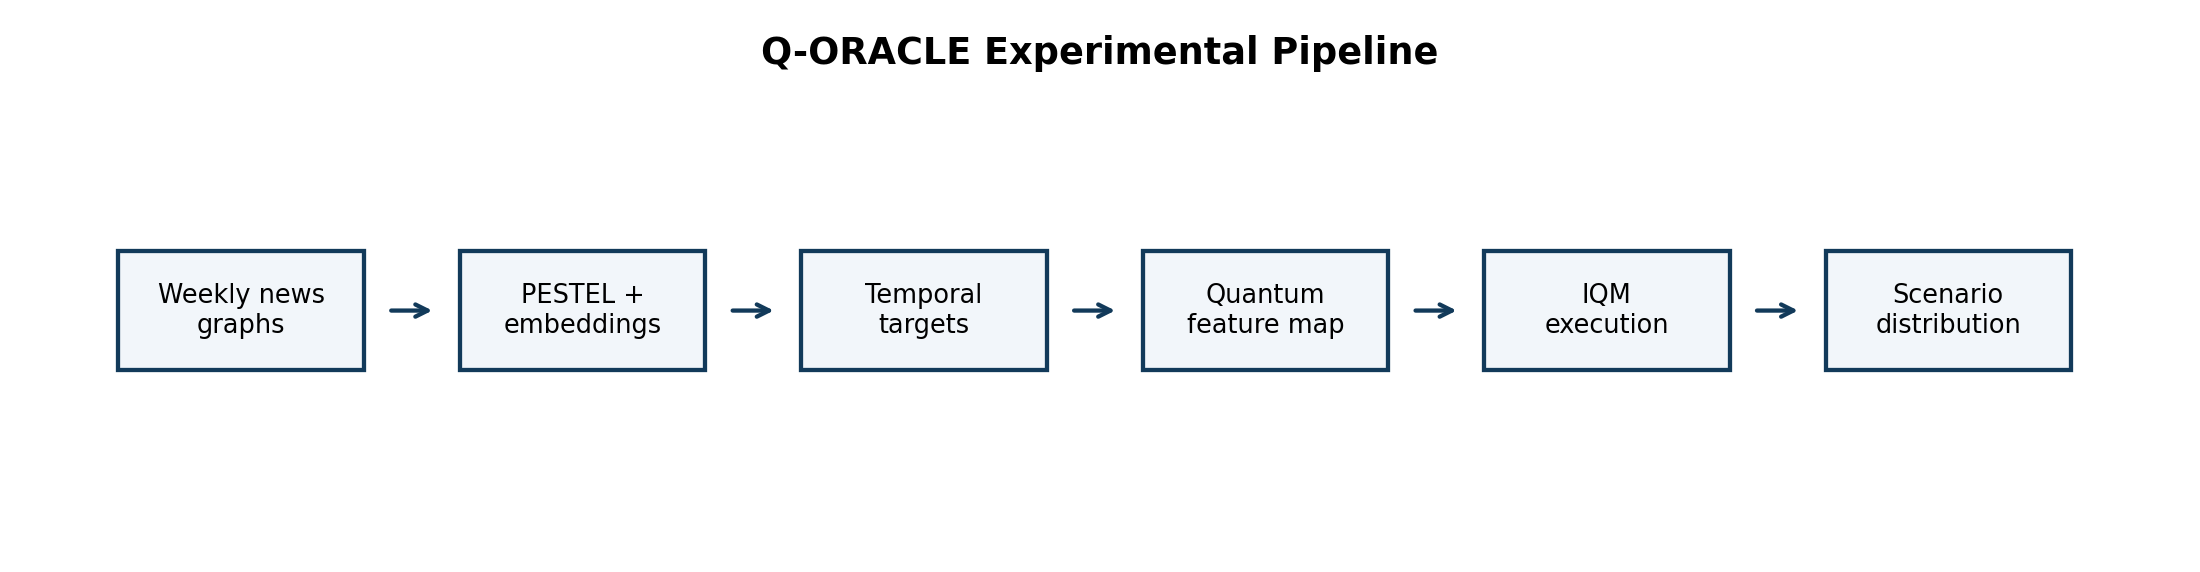
\includegraphics[width=0.92\textwidth]{figures/qoracle_pipeline.png}
\caption{Q-ORACLE experimental pipeline from news snapshots to quantum-sampled scenario probabilities.}
\label{fig:pipeline}
\end{figure*}

\subsection{Input Data}
The current artifact uses three weekly snapshots stored in the QuantumFinances hardware payload. Each week contains graph metadata, clusters, raw graph links and a normalized PESTEL vector:
\[
v_t = [P_t,E_t,S_t,T_t,Env_t,L_t]\in[0,1]^6.
\]
The latest run payload also contains an event vector and scenario probabilities produced by the Q-ORACLE scenario engine.

\subsection{PESTEL Timeline}
Figure~\ref{fig:pestel} shows the weekly trajectory used by the experiment. The values are not raw market data; they are normalized world-state features derived from clustered news snapshots. The latest vector is listed in Table~\ref{tab:pestel-latest}.

\begin{figure}[t]
\centering
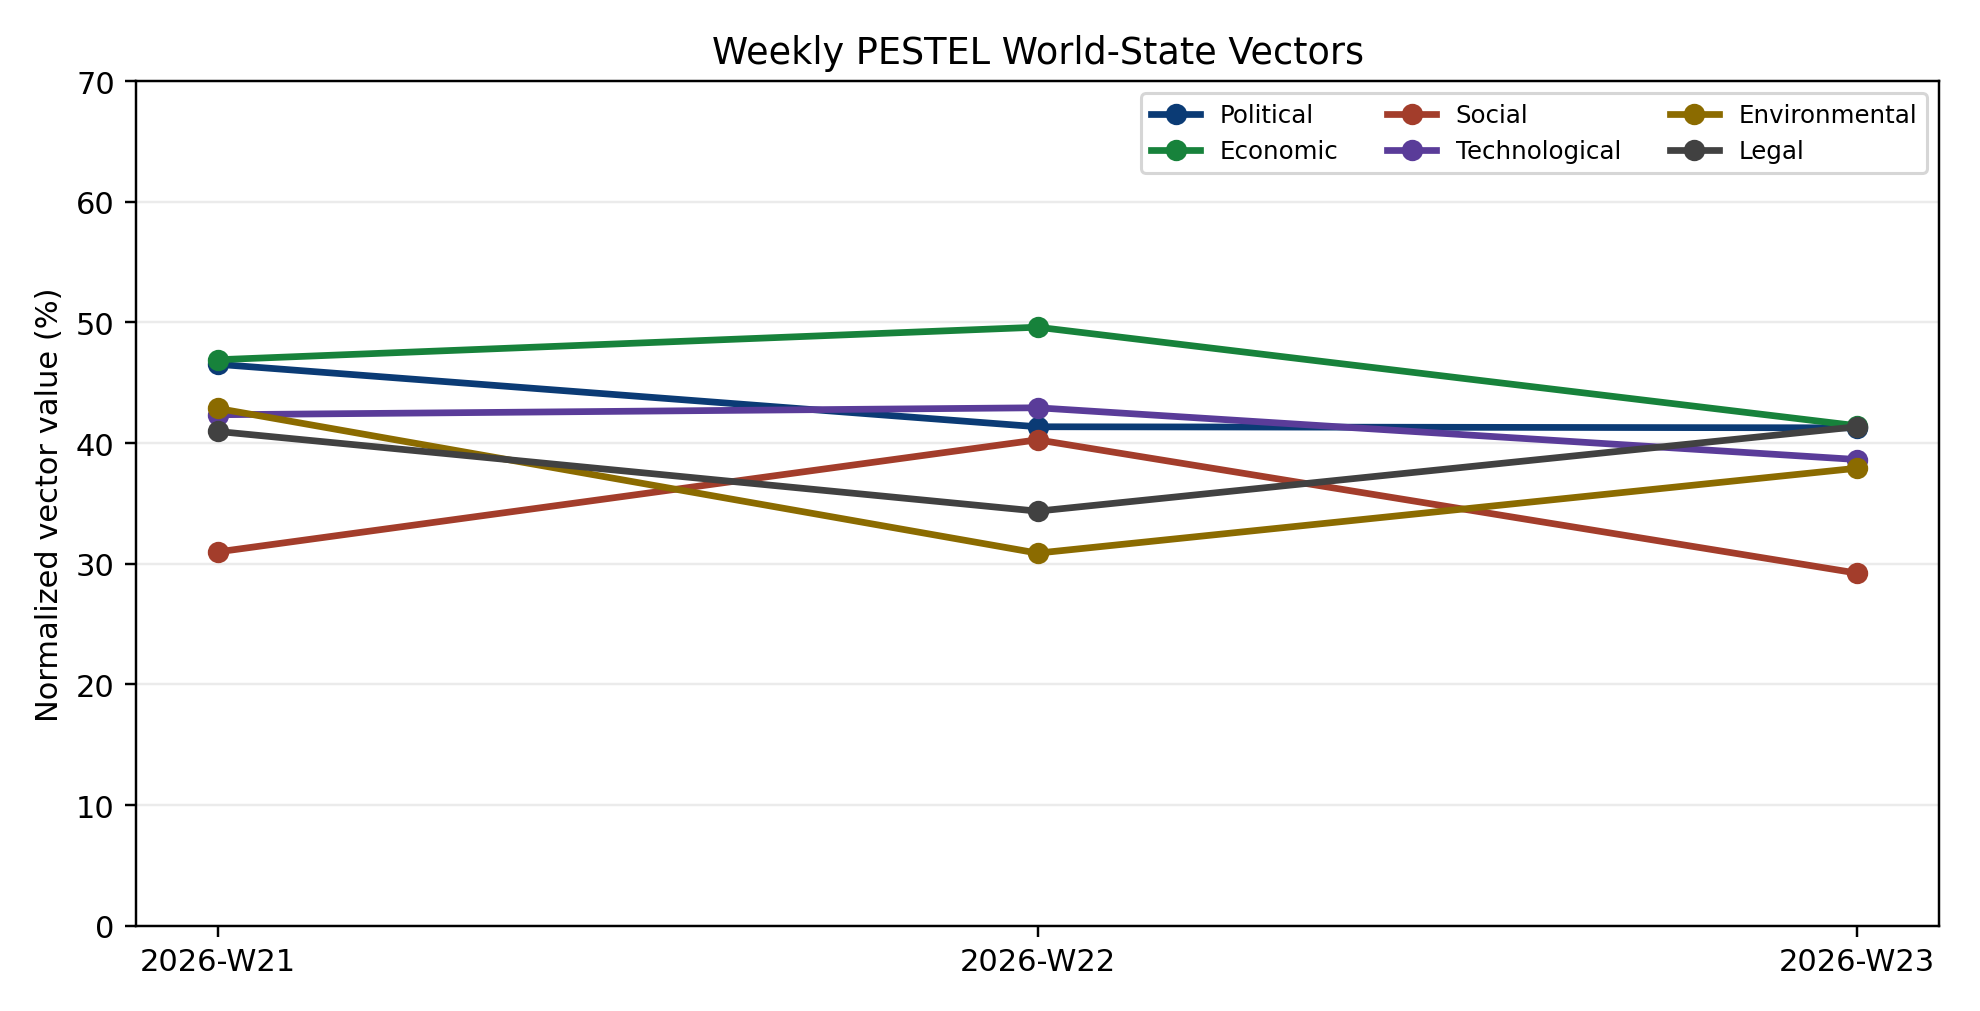
\includegraphics[width=\columnwidth]{figures/pestel_timeline.png}
\caption{Weekly PESTEL vectors for the current sample payload.}
\label{fig:pestel}
\end{figure}

\section{Temporal QML Method}
\subsection{Latent Compression}
To keep the QPU circuit small, the six-dimensional PESTEL vector is compressed into four latent features:
\[
z_t = [z^{PL}_t,z^{ET}_t,z^{SE}_t,z^{G}_t].
\]
The first three combine semantically paired PESTEL dimensions: political/legal, economic/technological and social/environmental. The fourth combines temporal trend and graph intensity:
\[
z^{G}_t=\mathrm{clip}(0.50+0.75\bar{\Delta}_t+0.35g_t),
\]
where \(\bar{\Delta}_t\) is the mean week-over-week PESTEL change and \(g_t\) is graph link intensity.

\subsection{Training Objective}
For each transition \(t\rightarrow t+1\), the model builds a four-class target distribution:
\[
y_t=[p_\mathrm{stable},p_\mathrm{up},p_\mathrm{down},p_\mathrm{uncertain}].
\]
The target uses event-vector alignment, weighted PESTEL similarity and volatility. The circuit output distribution \(q_\theta(z_t)\) is optimized using cross-entropy:
\[
\mathcal{L}(\theta)=-\sum_{t}\sum_{c} y_{t,c}\log q_{\theta,c}(z_t).
\]
Because the available history is short, the optimizer is deliberately simple: seeded local stochastic search over a compact 16-parameter ansatz. This makes the run reproducible and avoids overpresenting the result as a trained forecasting model.

\subsection{Circuit}
The circuit has four data qubits and two measured scenario bits. Each latent feature is encoded through \(R_y\) and \(R_z\) rotations. Two variational layers then apply per-qubit rotations and a ring of CNOT entanglers. The final two measured qubits define scenario classes:
\begin{align*}
00&=\mathrm{stable},&
01&=\mathrm{aligned\ up},\\
10&=\mathrm{aligned\ down},&
11&=\mathrm{uncertain}.
\end{align*}

\section{Implementation}
The implementation is contained in the Q-Fins repository. The temporal QML hardware script is:
\begin{center}
\small\texttt{quantum\_hardware/scripts/iqm\_temporal\_qml\_submit.py}
\end{center}
It consumes \texttt{latest\_run.json}, trains the variational parameters, writes a receipt and optionally submits to IQM Resonance through Qiskit-on-IQM. A batch runner,
\texttt{iqm\_batch\_qml\_experiments.py}, repeats the experiment over seeds and shot counts, writing JSON and CSV summaries.

The run command used for the verified temporal-QML experiment was:
\begin{center}
\scriptsize\texttt{iqm\_temporal\_qml\_submit.py --input latest\_run.json --shots 128 --iterations 60 --submit --wait}
\end{center}

\section{Hardware Results}
The temporal QML job was submitted to IQM Sirius and returned job ID:
\begin{center}
\small\texttt{019e9de9-956e-7622-ace6-80049a84a06c}.
\end{center}
The result contains 128 shots with counts shown in Table~\ref{tab:counts}. The local statevector distribution and hardware sample distribution are compared in Table~\ref{tab:qml-results} and Figure~\ref{fig:qmlcomparison}.


\begin{table}[t]
\centering
\small
\begin{tabular}{lrr}
\toprule
Class & Local QML & IQM hardware \\
\midrule
Stable & 49.4\% & 41.4\% \\
Aligned Up & 26.2\% & 20.3\% \\
Aligned Down & 9.4\% & 25.0\% \\
Uncertain & 15.0\% & 13.3\% \\
\bottomrule
\end{tabular}
\caption{Temporal QML scenario distribution. The local column is the statevector prediction after classical training; the hardware column is sampled from IQM Sirius.}
\label{tab:qml-results}
\end{table}

\begin{table}[t]
\centering
\small
\begin{tabular}{lr}
\toprule
Dimension & Latest value \\
\midrule
Political & 41.3\% \\
Economic & 41.4\% \\
Social & 29.2\% \\
Technological & 38.6\% \\
Environmental & 37.9\% \\
Legal & 41.4\% \\
\bottomrule
\end{tabular}
\caption{Latest weekly PESTEL vector used for feature encoding.}
\label{tab:pestel-latest}
\end{table}

\begin{table}[t]
\centering
\small
\begin{tabular}{lrr}
\toprule
Bitstring & Count & Share \\
\midrule
00 & 53 & 41.4\% \\
01 & 26 & 20.3\% \\
10 & 32 & 25.0\% \\
11 & 17 & 13.3\% \\
\bottomrule
\end{tabular}
\caption{Raw IQM temporal-QML hardware counts.}
\label{tab:counts}
\end{table}

\begin{table}[t]
\centering
\scriptsize
\begin{tabular}{lp{0.38\columnwidth}r}
\toprule
Experiment & Job ID & Shots \\
\midrule
Feature circuit & 019e9de2-2ab7-7653-9134-15e34fbe5926 & 128 \\
Temporal QML & 019e9de9-956e-7622-ace6-80049a84a06c & 128 \\
\bottomrule
\end{tabular}
\caption{Verified IQM hardware jobs available at paper-generation time.}
\label{tab:hardware-jobs}
\end{table}

\begin{table}[t]
\centering
\small
\begin{tabular}{lr}
\toprule
Batch mode & Dry-run \\
Records & 10 \\
Total shots & 960 \\
\bottomrule
\end{tabular}
\caption{Automatic temporal-QML batch summary used for the seed-sensitivity figure.}
\label{tab:batch-summary}
\end{table}

\begin{table}[t]
\centering
\scriptsize
\begin{tabular}{lp{0.50\columnwidth}}
\toprule
Semantic embedding model & \path{intfloat/multilingual-e5-large-instruct} \\
Embedding dimension & 1024 \\
Hardware jobs & 18 \\
Total hardware shots & 13824 \\
Latent qubits tested & 8, 10, 12 \\
\bottomrule
\end{tabular}
\caption{Semantic-embedding QML batch configuration.}
\label{tab:semantic-config}
\end{table}

\begin{table*}[t]
\centering
\small
\begin{tabular}{rrrrrrr}
\toprule
Qubits & Records & Shots & Stable & Event aligned & Event divergent & Uncertain \\
\midrule
8 & 6 & 4608 & 32.3\% & 29.3\% & 19.1\% & 19.2\% \\
10 & 6 & 4608 & 29.3\% & 27.6\% & 21.8\% & 21.2\% \\
12 & 6 & 4608 & 32.7\% & 31.4\% & 18.0\% & 17.9\% \\
\bottomrule
\end{tabular}
\caption{Mean IQM Sirius hardware distributions for the 1024-dimensional semantic-embedding QML batch.}
\label{tab:semantic-batch}
\end{table*}

\begin{table}[t]
\centering
\small
\begin{tabular}{lr}
\toprule
Class & Overall mean \\
\midrule
Stable & 31.5\% \\
Event Aligned & 29.4\% \\
Event Divergent & 19.7\% \\
Uncertain & 19.4\% \\
\bottomrule
\end{tabular}
\caption{Aggregate distribution across all semantic-embedding QML hardware jobs.}
\label{tab:semantic-overall}
\end{table}


\begin{figure}[t]
\centering
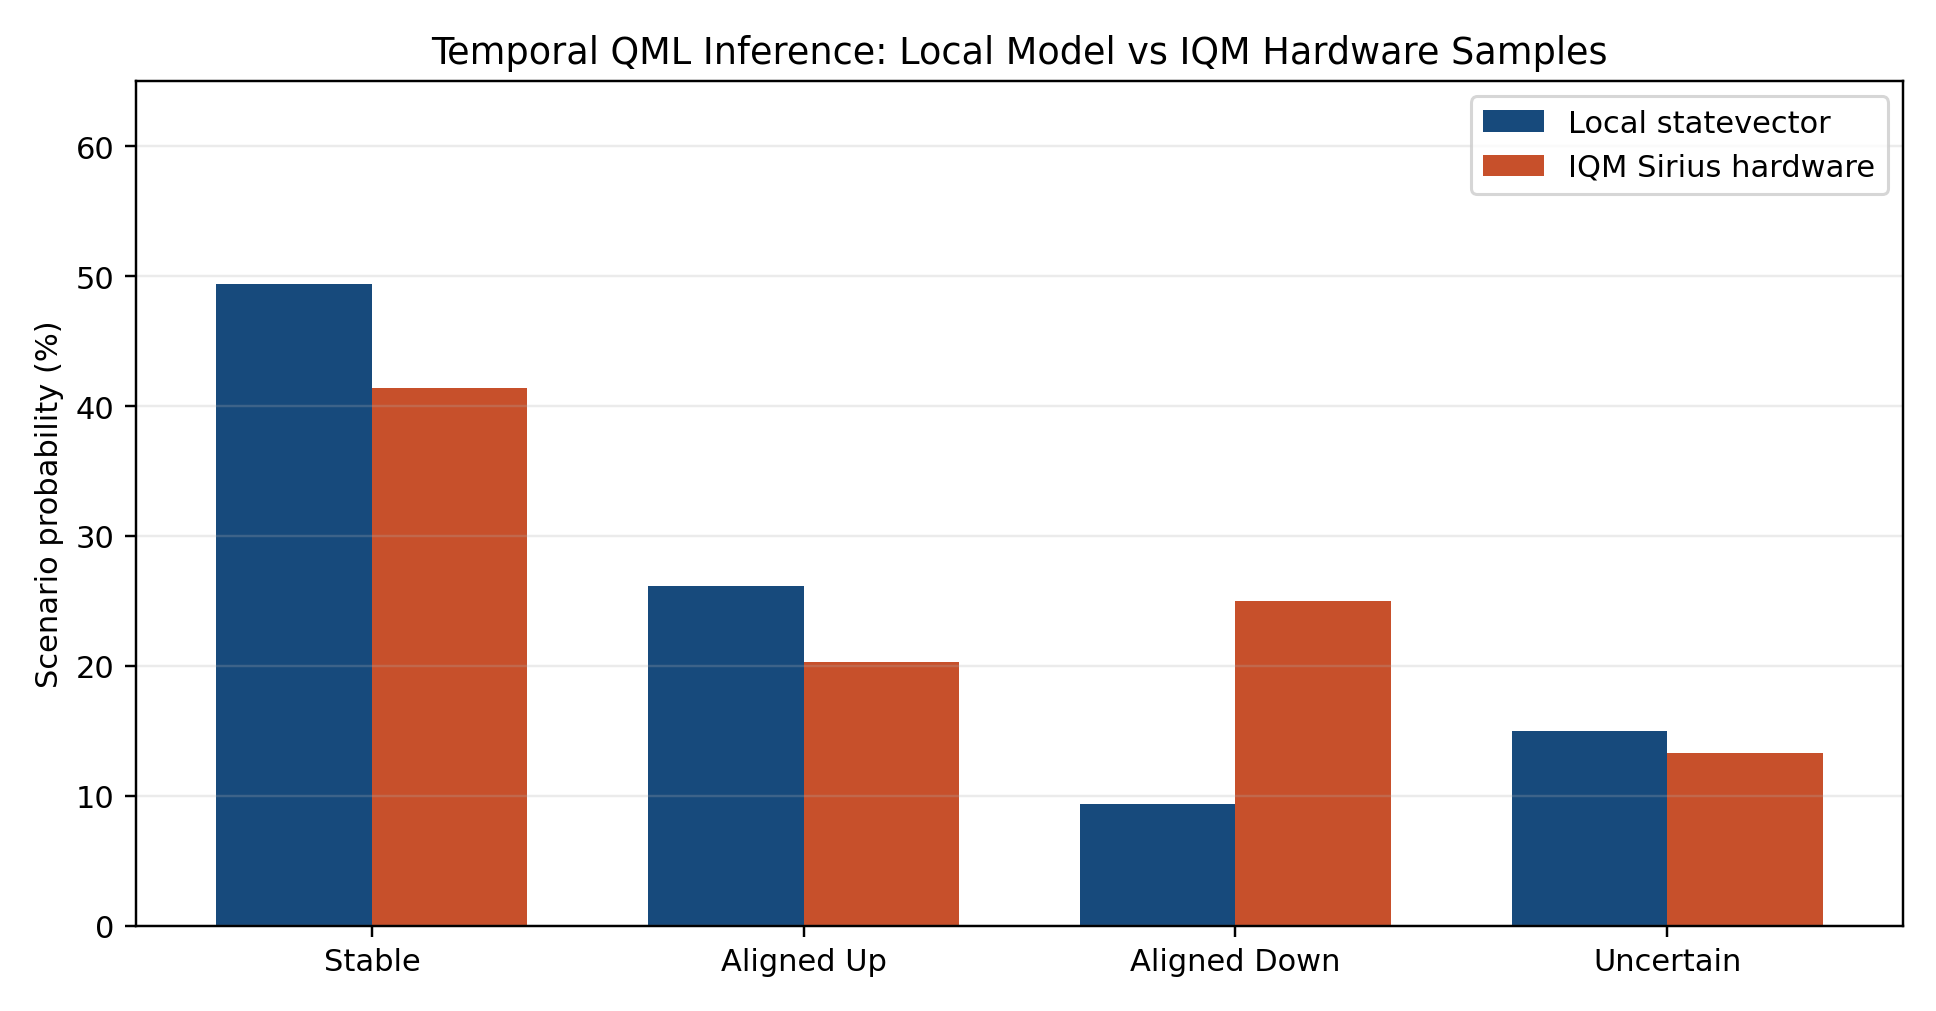
\includegraphics[width=\columnwidth]{figures/qml_local_vs_hardware.png}
\caption{Temporal QML local inference probabilities compared with IQM Sirius hardware samples.}
\label{fig:qmlcomparison}
\end{figure}

\begin{figure}[t]
\centering
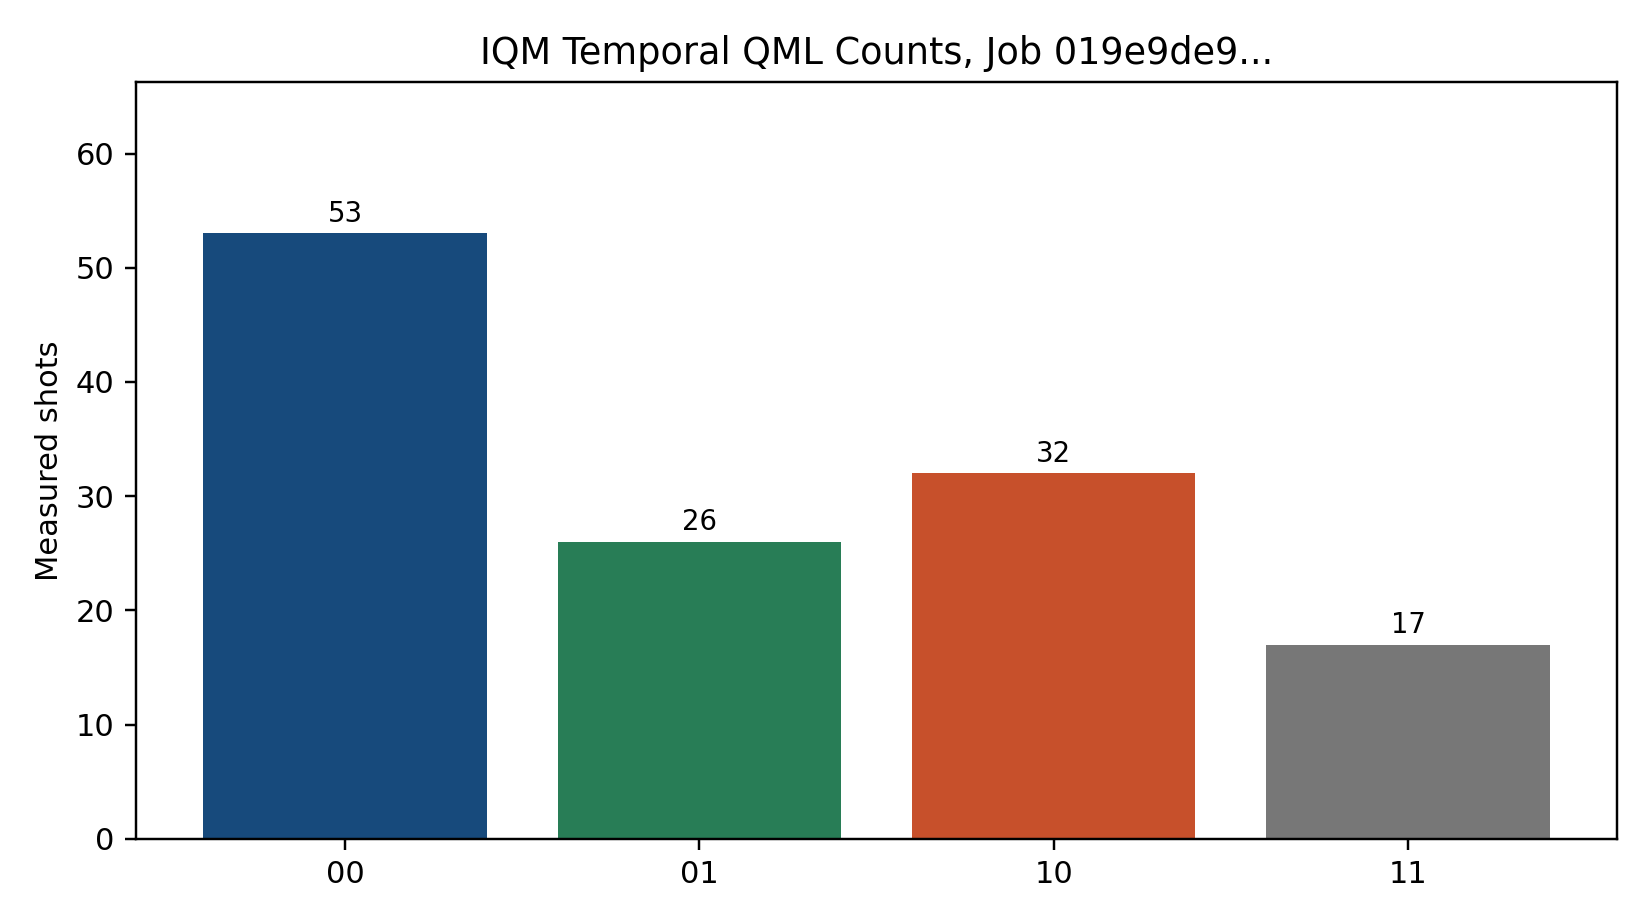
\includegraphics[width=\columnwidth]{figures/iqm_qml_counts.png}
\caption{Raw IQM temporal QML counts for the verified hardware job.}
\label{fig:counts}
\end{figure}

\section{Batch Experiments}
The batch runner was executed in dry-run mode over five seeds and two shot settings, producing ten reproducible training/inference records. Figure~\ref{fig:batch} shows seed sensitivity for the 128-shot configuration. The batch script is hardware-capable: when \texttt{IQM\_TOKEN} is available and \texttt{--submit --wait} are provided, each record becomes a submitted IQM job and is written to the same summary format.

\begin{figure}[t]
\centering
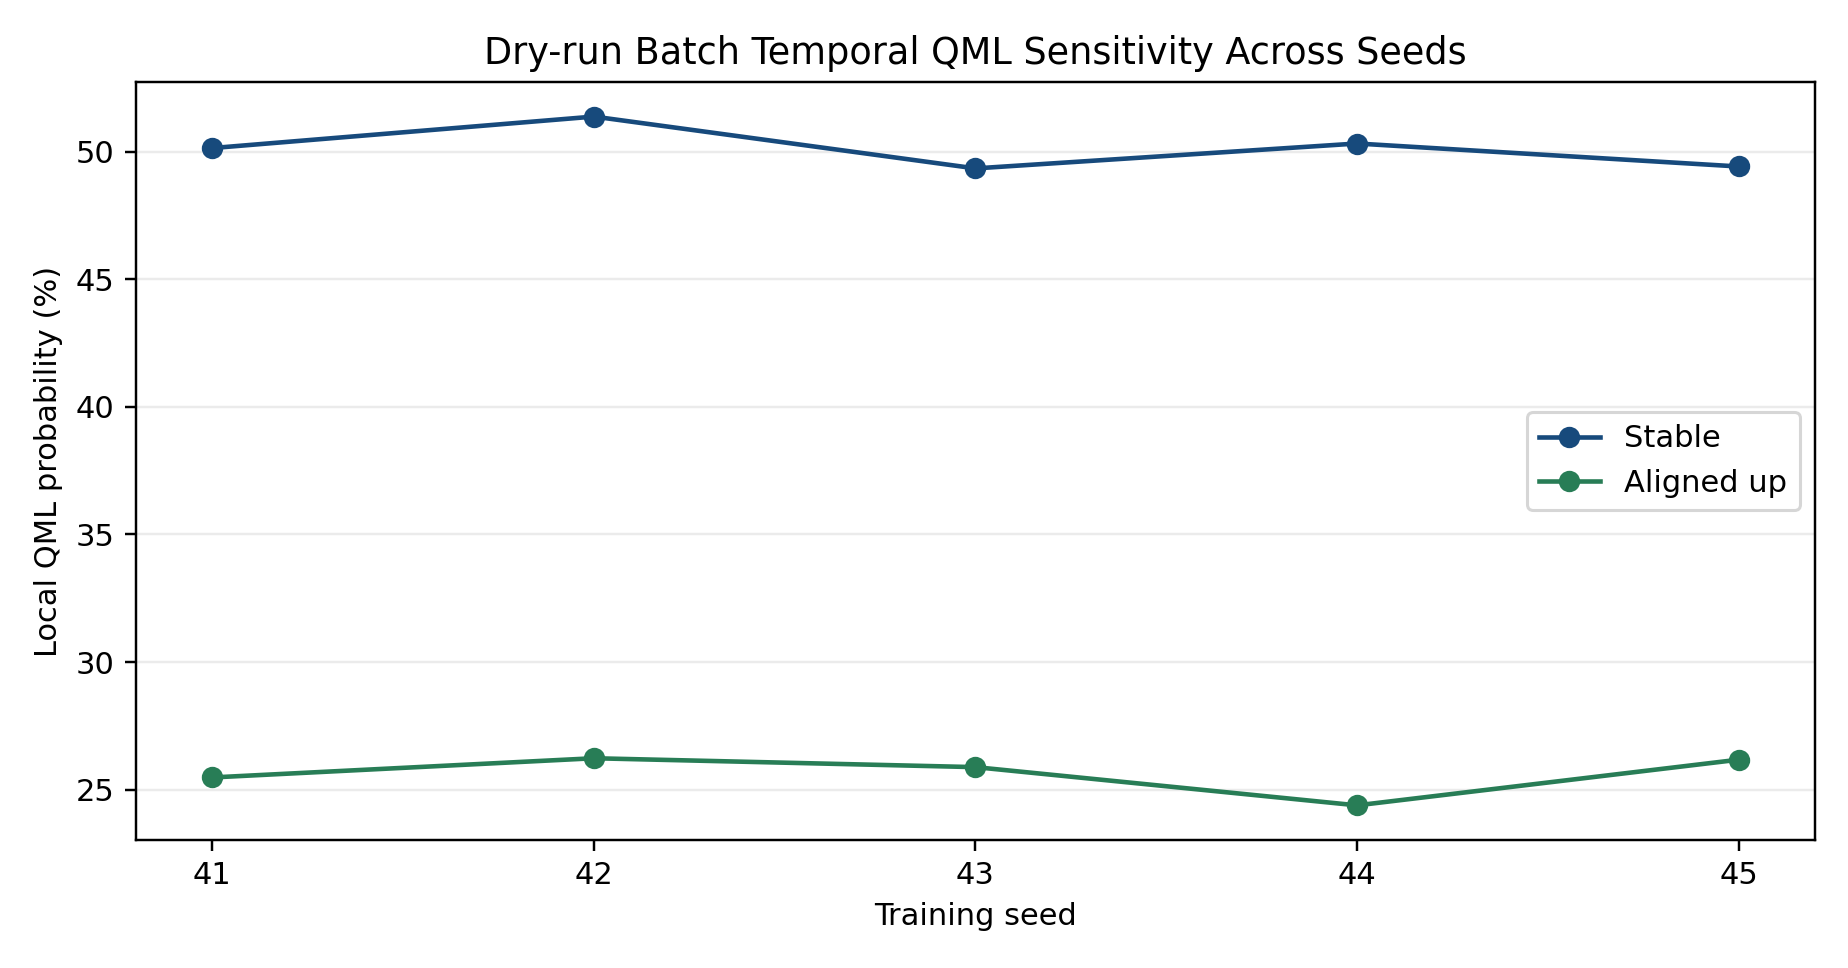
\includegraphics[width=\columnwidth]{figures/qml_batch_seed_sensitivity.png}
\caption{Dry-run batch sensitivity of local temporal-QML probabilities across seeds.}
\label{fig:batch}
\end{figure}

\section{Screenshots and Reproducibility Artifacts}
Figure~\ref{fig:screens} captures the working prototype interface and IQM Resonance access point used for hardware execution. These screenshots are not used as scientific evidence; they document the operational environment for the hackathon artifact.

\begin{figure*}[t]
\centering
\begin{subfigure}{0.48\textwidth}
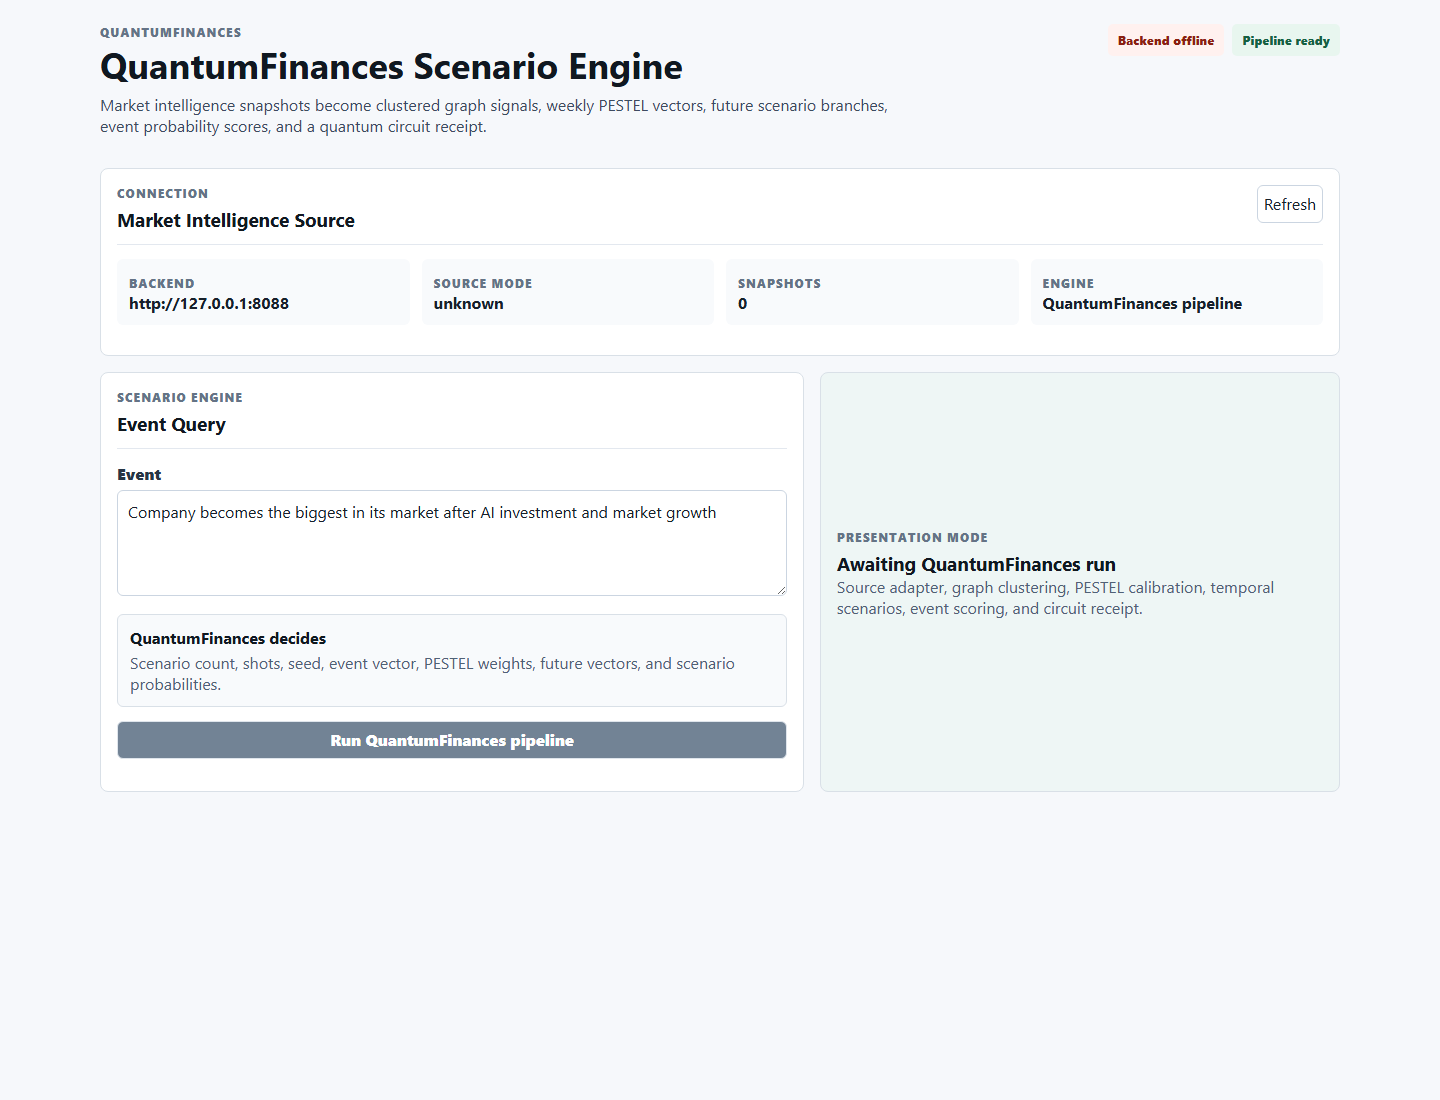
\includegraphics[width=\linewidth]{figures/qoracle_app_dashboard.png}
\caption{Q-ORACLE scenario interface.}
\end{subfigure}
\hfill
\begin{subfigure}{0.48\textwidth}
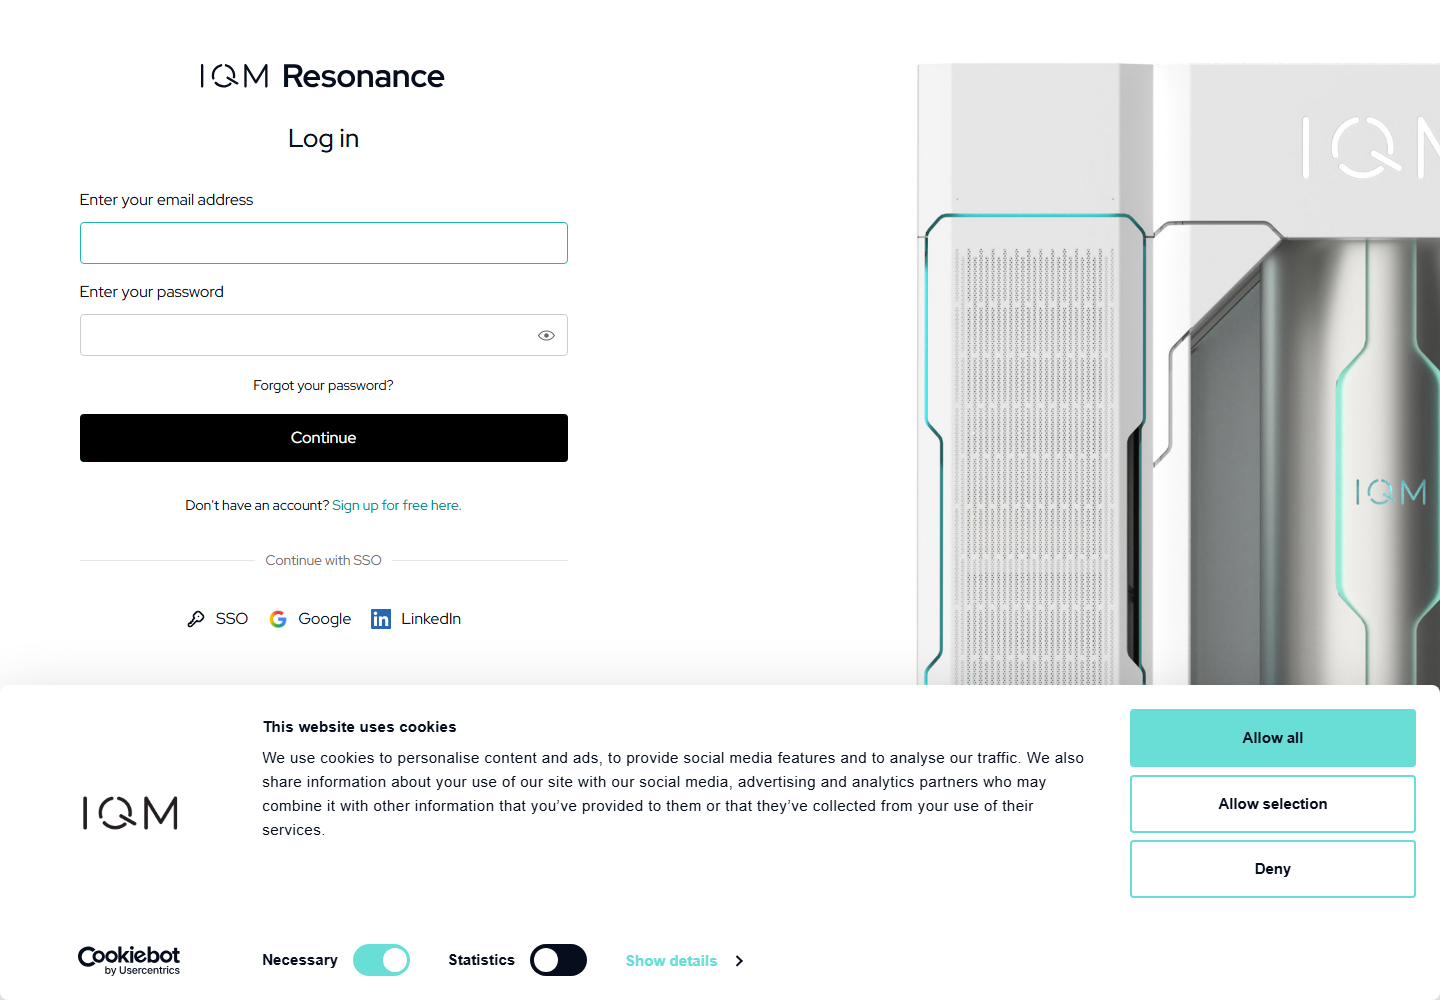
\includegraphics[width=\linewidth]{figures/iqm_resonance_public.png}
\caption{IQM Resonance public access page.}
\end{subfigure}
\caption{Screenshots included for reproducibility and presentation context.}
\label{fig:screens}
\end{figure*}

\section{Discussion}
The hardware run is informative in three ways. First, it verifies that the ORACLE/PESTEL pipeline can produce a circuit that survives provider transpilation and executes on a real superconducting QPU. Second, the local-vs-hardware comparison exposes sampling and hardware effects directly instead of hiding them behind a simulated receipt. Third, the result gives a concrete scenario distribution that can be displayed in the application as a hardware-backed QML branch.

The local model predicted the stable branch as dominant, while the hardware samples reduced the stable share and increased the aligned-down branch. With only 128 shots and one hardware run, this should be interpreted as an empirical sample from a noisy near-term device, not as a calibrated probability of a real-world event.

\section{Limitations}
The most important limitation is data scale: three weekly snapshots provide only two transition examples. This is enough for a hackathon hardware demonstration but not enough for statistical validation. The PESTEL vectors are also derived from sample snapshots rather than a large live production archive. Additionally, the circuit is shallow by design; larger ansatzes may be more expressive but are harder to train and noisier on near-term hardware. Finally, the event probability is a scenario compatibility score, not investment advice or a verified forecast.

\section{Conclusion}
Q-ORACLE demonstrates an end-to-end path from auditable news graph foresight to temporal QML execution on real IQM hardware. The prototype turns weekly PESTEL vectors into transition targets, trains a compact variational circuit and samples the resulting scenario register on IQM Sirius. The main contribution is not predictive accuracy, but a reproducible architecture for linking narrative intelligence, temporal vector modeling and quantum hardware receipts.

\begin{thebibliography}{9}
\bibitem{oracle2025}
L. Kharlashkin, E. Morooka, Y. Tereshchenko, and M. Hämäläinen.
\newblock ORACLE: Time-Dependent Recursive Summary Graphs for Foresight on News Data Using LLMs.
\newblock arXiv:2512.15397, 2025.

\bibitem{mlpestel2024}
K. Alnajjar and M. Hämäläinen.
\newblock MLPestel: The New Era of Forecasting Change in the Operational Environment of Businesses Using LLMs.
\newblock Centria University of Applied Sciences, 2024.

\bibitem{kaushik2022onestep}
P. Kaushik, S. Pramanik, M. G. Chandra, and C. V. Sridhar.
\newblock One-Step Time Series Forecasting Using Variational Quantum Circuits.
\newblock arXiv:2207.07982, 2022.

\bibitem{horowitz2022hamiltonian}
H. Horowitz, P. Rao, and S. K. Radha.
\newblock A Quantum Generative Model for Multi-Dimensional Time Series Using Hamiltonian Learning.
\newblock arXiv:2204.06150, 2022.

\bibitem{chittoor2024qultsf}
H. H. S. Chittoor, P. R. Griffin, A. Neufeld, J. Thompson, and M. Gu.
\newblock QuLTSF: Long-Term Time Series Forecasting with Quantum Machine Learning.
\newblock arXiv:2412.13769, 2024.

\bibitem{fellner2025benchmark}
T. Fellner, D. Kreplin, S. Tovey, and C. Holm.
\newblock Quantum vs. Classical: A Comprehensive Benchmark Study for Predicting Time Series with Variational Quantum Machine Learning.
\newblock arXiv:2504.12416, 2025.

\bibitem{schuld2019hilbert}
M. Schuld and N. Killoran.
\newblock Quantum Machine Learning in Feature Hilbert Spaces.
\newblock Physical Review Letters, 122:040504, 2019.

\bibitem{larocca2024barren}
M. Larocca et al.
\newblock A Review of Barren Plateaus in Variational Quantum Computing.
\newblock arXiv:2405.00781, 2024.
\end{thebibliography}

\end{document}
